\section{Motivation}

% SLAM
Robots often have to act in an unknown environment. For that, a robot has to recognize the environment and locate itself in it. For example, an actor wants to find the dishwasher to clean up the kitchen. This problem is also known as simultaneous localization and mapping (SLAM) in the context of robotics. Common approaches using discrete landmarks recognized by the robot to set up a landmark map of the environment (see figure \ref{fig:grisetti_slam_example}). With this map of landmarks, it's possible to estimate the position of the robot. A typical example of landmarks are features from images, which are taken by a camera from the robot.

% From discrete to continuous
For SLAM there are a variety of use cases but there are also scenarios where it's not possible to obtain landmarks that are suitable for SLAM approaches. For example, at the sea, water is usually muddy and cameras would only see over a short distance. There it wouldn't be possible to extract image features suitable for SLAM approaches. That's where scientists switched from discrete landmarks to continuous functions given by physical phenomena. A common approach is to use the magnetic field for indoor localization. This is also a good example to show also what performance such approaches could have.

% Vision
But it's not only a workaround to use SLAM in situations, where discrete landmarks are not possible to obtain. Continuous approaches could be as good as discrete ones and in combination, they could be even better. Also, when it comes to costs if the aim of a robot is to measure physical phenomena, why don't use this data for SLAM instead of buying a camera and more expensive hardware for real-time feature extraction of the images.

% Science question
There is a huge potential of SLAM with continuous functions and the science community is only at the beginning. This project wants to examine if an actor could locate itself in an unprepared unknown environment only by using a microphone, speaker and inertial measurement unit (IMU). For that, the speaker sends out a signal which is received by the microphone. But the signal will be changed mainly because of interference of the signal with the room. 

% Aims and Tasks
One Task is now to derive a continuous function from the microphone signal. For that, the room will be treated as an electrical system. The signal from the speaker will be the input and the microphone signal the output of the system. So an impulse response could be calculated. This concept is already known as the room impulse response (RIR). Based on that, various continuous functions have to be validated which one is the best for indoor SLAM approaches. For example, using only the ten highest peaks of the RIR. But before that, data has to be recorded for analysis, test and validation purposes. At the end of this project, the performance of this indoor SLAM approach should be compared to other acoustic SLAM approaches and also to other indoor SLAM approaches with other physical phenomena like the magnetic field.

\begin{figure}[h!]
	\centering
	\captionsetup{justification=centering,margin=0.5cm}
	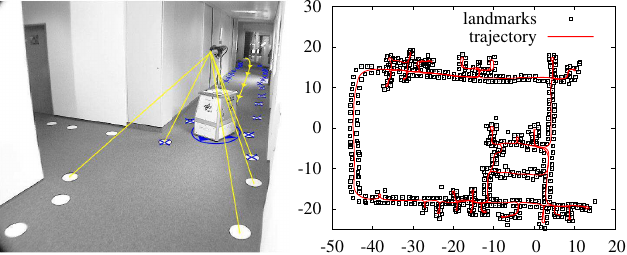
\includegraphics[width=0.935\textwidth]{images/grisetti_slam_example.png}
	\caption{
		An illustration for SLAM with a prepared environment for the robot. Landmarks are mounted on the floor which the robot can recognize (left image). The generated map is shown on the right \cite{grisetti_tutorial_2010}.
	}
	\label{fig:grisetti_slam_example}
\end{figure}